\documentclass{article}
\usepackage{graphicx} 
\usepackage{listings}
\usepackage{xcolor}
\usepackage{url}
\usepackage{hyperref}

\lstdefinestyle{python}{
    language=Python,        
    basicstyle=\ttfamily,    
    keywordstyle=\color{blue},   
    stringstyle=\color{red},     
    commentstyle=\color{green}, 
    morekeywords={self},    
    breaklines=true,        
    numbers=left,           
    numberstyle=\tiny\color{gray}, 
    captionpos=b           
}

\begin{document}
\begin{titlepage}
    \centering
    \vfill
    \Huge Monitoreo del Tráfico Aéreo: Análisis en Tiempo Real\\[1cm]
    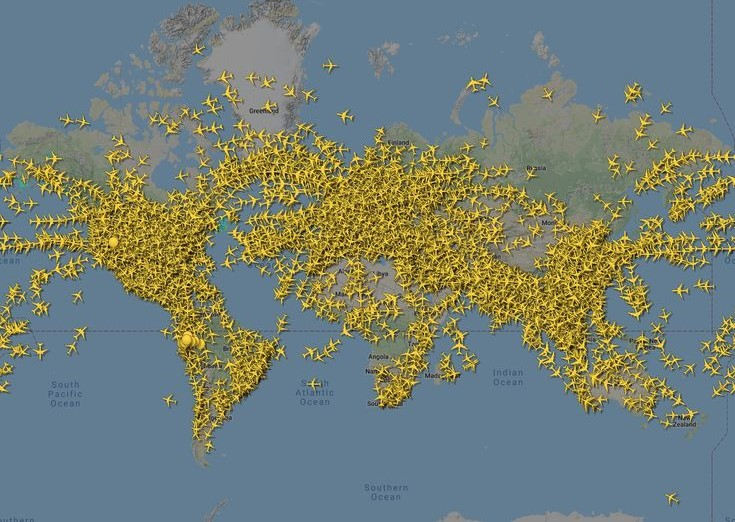
\includegraphics[width=0.9\textwidth]{presentation.jpg}  
    \vfill
    \Large Autores: \\Marian Aguilar Tavier. \\  Jennifer de la C. Sánchez. \\[1cm]
    \Large Febrero, 2025
    \vfill
\end{titlepage}
\tableofcontents
\newpage
\setcounter{secnumdepth}{0}

\section{Introducción}
Hoy en día, la cantidad de datos generados en un instante de tiempo muy pequeño es prácticamente innumerable, provenientes de múltiples fuentes. De esta forma surge lo que se conoce como \textit{Big Data}.
El procesamiento y análisis de grandes volúmenes de datos de manera eficiente permite obtener información valiosa que optimiza procesos, predice tendencias y ofrece soluciones a problemas complejos, independientemente del ámbito de aplicación.

De esta forma, una de las aplicaciones del Big Data radica en el análisis de datos referentes al tráfico aéreo. Este enfoque no solo permite el monitoreo en tiempo real de las operaciones aéreas, sino que también facilita el desarrollo de análisis más complejos. De esta manera, es posible predecir retrasos, identificar picos de actividad, detectar temporadas con mayor tráfico aéreo, etcétera.

Debido a la relevancia y utilidad que tiene este tema, este proyecto tiene como objetivo desarrollar un sistema para la captura, análisis y almacenamiento de datos en tiempo real sobre el tráfico aéreo a nivel global. El sistema brindará información actualizada sobre las operaciones aéreas, posibles retrasos en los vuelos y condiciones meteorológicas que puedan afectar la trayectoria de las aeronaves.  

Para ello, se emplearán tecnologías propias de BigData como Apache Kafka, Hadoop Distributed File System(HDFS), junto con Python y Docker para garantizar un entorno aislado y bien estructrurado que optimice la captura, el almacenamiento y el análisis de datos. 
\newpage

\section{Ingesta de datos}

\subsection{API utilizada}

Para la ingesta de los datos en este caso se ha empleado la API de OpenSky Network \cite{Schaefer2014}. La misma proporciana datos de aviación en tiempo real de Automatic Dependent Surveillance-Brodcast (ADS-B) que se recopilan a
partir de una red de sensores que se encuentran ubicados en todo el mundo.

El acceso a estos datos es gratuito. La API genera vectores de estado para cada aeronave, que incluyen detalles como el identificador ICAO, el llamado (callsign), el país de origen, la posición en tiempo, la velocidad de la aeronave y la última hora de contacto.

Se pueden realizar consultas para obtener información sobre vuelos específicos o todos los vuelos dentro de un intervalo de tiempo determinado. Esto incluye la capacidad de filtrar por aeronave específica.
Además permite acceder a un historial de vuelos hasta 30 días atrás, lo que es útil para análisis posteriores y seguimiento de aeronaves.

Es importante destacar que no proporciona datos comerciales de vuelo como horarios de aeropuertos, retrasos o información adicional que no pueda derivarse del contenido de los datos ADS-B.

Para acceder a la API y a todos los vuelos en tiempo real se ha utilizado la url: \url{https://opensky-network.org/api/states/all}.

\subsection{Apache Kafka para la ingesta}
\subsubsection{¿Qué es Apache Kafka?}

Apache Kafka es una plataforma de transmisión distribuida diseñada para manejar flujos de datos en tiempo real de manera eficiente, escalable y confiable \cite{KafkaDocumentation}. Gracias a su arquitectura basada en discos y su enfoque en operaciones secuenciales, Kafka puede manejar millones de mensajes por segundo con una latencia extremadamente baja, lo que lo convierte en una solución ideal para aplicaciones de alto rendimiento.
Tiene numerosos casos de uso, como la transmisión distribuida, el procesamiento de flujos, la integración de datos y la mensajería de publicación/suscripción.

Para comprender como funciona Apache Kafka es necesario comprender algunos conceptos fundamentales:

\begin{itemize}
    \item \textbf{Topic: }es básicamente una categoría o un nombre de fuente en el que se almacenan y publican mensajes durante las operaciones. Los mensajes son en su mayoría matrices de bytes que pueden almacenar cualquier objeto en cualquier formato. Representa una unidad de datos que encapsula un evento. Cada tema en Kafka está dividido en particiones, que son subconjuntos del tema distribuidos entre varios nodos del clúster, permitiendo el manejo simultáneo de múltiples flujos de datos y garantizando la escalabilidad.
    \item \textbf{Producer: }Los productores son componentes del sistema que generan datos y los publican en uno o más temas en Kafka. Estos productores tienen la capacidad de etiquetar los mensajes con claves específicas, lo que facilita la organización y distribución de los datos dentro de las particiones del tema.
    \item \textbf{Consumer: } los consumidores son aplicaciones que se suscriben a los temas para procesar los mensajes a medida que se publican. Los consumidores pueden trabajar de forma independiente o como parte de un grupo, donde la carga de trabajo se distribuye entre múltiples instancias para maximizar la eficiencia.
    \item \textbf{Broker: }El clúster de Kafka está compuesto por múltiples brokers, que son nodos responsables de almacenar y administrar los datos de los temas. Cada partición dentro de un tema tiene un líder, que es el broker encargado de manejar las solicitudes de lectura y escritura, mientras que las réplicas de las particiones se almacenan en otros brokers para garantizar la disponibilidad en caso de fallos. Esta replicación de particiones es una de las principales características que hacen de Kafka un sistema tolerante a fallos, ya que permite que el sistema continúe operando incluso si uno o varios brokers fallan.

\end{itemize}

Al dividir un registro en particiones, Kafka puede escalar horizontalmente los sistemas. Como tal, Kafka modela los eventos como pares clave-valor. Internamente, las claves y los valores son solo secuencias de bytes, pero externamente en el lenguaje de programación de elección, a menudo son objetos estructurados representados en el sistema de tipos de su lenguaje. Kafka llama a la traducción entre tipos de lenguaje y serialización y deserialización de bytes internos. El formato serializado suele ser JSON, JSON Schema, Avro o Protobuf.

\subsubsection{¿Por qué utilizarlo en este caso?}

En el caso del tráfico aéreo y el monitereo de aviones, estamos en presencia de datos altamente dinámicos, por lo que es necesario tener acceso en tiempo real al estado de cada una de las aeronaves en todo el mundo, y Kafka es una herramienta ideal para lograrlo.

El número de aviones en vuelo puede variar significativamente dependiendo de la hora del día, el día de la semana o la temporada. Kafka permite escalar horizontalmente el sistema al agregar más brokers al clúster, garantizando que pueda manejar un incremento en la cantidad de datos sin problemas, en especial durante los horarios o temperadas picos de vuelo. Además se evita la pérdida de datos debido a su fuerte tolerancia a fallos en caso de interrupciones en la red u otro tipo de fallo en particular.

El uso de Kafka en este caso también facilita la integración con otras herramientas y tecnologías del ecosistema de big data, como Apache Spark, para el análisis en tiempo real, o HDFS, para el almacenamiento a largo plazo de datos históricos.

\subsection{Despliegue de Kafka con Docker y Docker Compose}

Luego de explicar los conceptos fundamentales que permiten comprender el funcionamiento de Apache Kafka, procedemos a explicar cómo se realizó finalmente este proceso de ingesta. Para ello, se utilizó Docker y Docker Compose, que permitieron una implementación eficiente y escalable del sistema.

Utilizamos Docker para crear contenedores que encapsulan Apache Kafka y Zookeeper, asegurando un entorno de ejecución consistente y simplificando la configuración. Con Docker Compose, pudimos definir y administrar estos contenedores de manera más sencilla y automatizada a través del archivo `docker-compose.yml`.

Este archivo incluye servicios para Apache Kafka, Zookeeper y Hadoop, especificando detalles como las imágenes de Docker a utilizar, los puertos expuestos, las variables de entorno necesarias y los volúmenes para persistencia de datos. Esta configuración permite crear un entorno de ejecución aislado y replicable, simplificando la gestión de la infraestructura y reduciendo los riesgos asociados a la configuración manual.

Una vez configurado correctamente el archivo de configuración de Docker, y cargada todas sus imágenes se inicializó el contenedor que se encargaría de llevar a cabo este proceso mediante el comando `docker compose up` y dentro de este se ejecuta todo lo que se explicará en la siguiente sección.

\subsection{Captura de los datos}

Para el proceso de captura de datos se utilizó Apache Kafka junto con la biblioteca \textit{kafka-python} \cite{KafkaPython}.

Se creó un archivo "producer.py" encargado de obtener los datos en tiempo real de la API  y enviarlos al clúster de Kafka.Estos datos se envían de forma continua a un topic en específico, para el cual se creó el topic `Air\_Traffic`, permitiendo una ingesta constante y actualizada de información sobre el estado de los vuelos.
Primero, se configura una instancia de KafkaProducer que se conecta al servidor de Kafka en localhost:9092. Este producer se encarga de serializar los datos en formato JSON antes de enviarlos. La configuración se realiza definiendo las propiedades de conexión y el serializador de valores.

\begin{lstlisting}[style=python]
from kafka import KafkaProducer
import json

producer = KafkaProducer(
    bootstrap_servers=['localhost:9092'],
    value_serializer=lambda x: json.dumps(x).encode('utf-8')
    )
\end{lstlisting}

Luego se implementó la función `fetch\_data`, que realiza solicitudes periódicas a la API de OpenSky-Network para obtener información sobre el estado de las aeronaves. Cada solicitud utiliza el protocolo HTTP, y los datos recibidos se procesan en formato JSON, lo que permite una integración directa con Kafka y otros componentes del sistema.
Una vez capturados, los datos se publican en el tema `Air\_Traffic` utilizando el método `send`, y se garantiza su envío inmediato mediante el uso del método `flush`. Este procedimiento asegura que no haya retrasos significativos en la transmisión de información, lo cual es crucial para aplicaciones en tiempo real como esta.

Luego de implementar el producer, se configuró el consumer que será el encargado de suscribirse al topic creado y leer los mensajes en tiempo real. Una vez que el consumer se suscribe a "Air Traffic"(topic) este deserializa los datos recibidos en formato json, asegurando que sean legibles y puedan ser procesados de manera eficiente.

\begin{lstlisting}[style=python]
from kafka import KafkaConsumer
import json

consumer = KafkaConsumer(
    'Air_Traffic',
    bootstrap_servers=['localhost:9092'],
    auto_offset_reset='earliest',
    value_deserializer=lambda x: json.loads(x.decode('utf-8'))
)
\end{lstlisting}

Una de las principales ventajas de utilizar consumidores de Kafka es su capacidad para operar de manera distribuida, lo que permite procesar grandes volúmenes de datos dividiendo la carga entre múltiples instancias. Esto garantiza que el sistema pueda escalar de forma eficiente según las necesidades.
Además por su naturaleza desacoplada los productores no dependen de los consumidores para operar, y los datos permanecen almacenados temporalmente en Kafka hasta que los consumidores estén listos para procesarlos, lo que no solo mejora la resiliencia del sistema, sino que también permite una mayor flexibilidad al integrar nuevos componentes o funcionalidades sin interrumpir el flujo de datos existente.

\section{Almacenamiento de datos}

\subsection{Hadoop Distributed File System(HDFS)}

HDFS es un sistema de archivos distribuido diseñado para almacenar grandes volúmenes de datos en un entorno distribuido y manejar de manera eficiente aplicaciones que requieren un procesamiento intensivo de datos.\cite{HadoopHDFS}

Utiliza una arquitectura distribuida que divide los datos en bloques de tamaño fijo y los distribuye entre varios nodos en un clúster. Una de sus características más importante es su  tolerancia a fallos, ya que cada bloque de datos se replica en múltiples nodos para garantizar la disponibilidad de los datos incluso si uno o varios nodos fallan. Por defecto, cada bloque tiene tres réplicas, aunque este número es configurable según las necesidades del sistema.

La arquitectura de HDFS sigue un modelo maestro-esclavo compuesto por el Namenode, que actúa como maestro, y los Datanodes, que son los nodos esclavos. El Namenode administra el sistema de archivos, gestionando metadatos como la estructura de directorios, la ubicación de los bloques y las políticas de replicación, mientras que los Datanodes almacenan físicamente los bloques de datos y ejecutan las operaciones de lectura y escritura según las instrucciones del Namenode.

Cuando un cliente escribe un archivo, este se divide en bloques que se envían a diferentes Datanodes, siguiendo las políticas de replicación establecidas. El Namenode registra las ubicaciones de estos bloques. En el caso de una lectura, el cliente consulta al Namenode para obtener la ubicación de los bloques y accede directamente a los Datanodes para leerlos. Si un nodo falla, el sistema replica automáticamente los bloques desde las copias disponibles en otros nodos para garantizar la continuidad del servicio.

\subsection{HDFS y Docker}

Como en el caso de la ingesta, se utilizó Docker con HDFS para crear un entorno aislado, portable y escalable que facilite tanto el desarrollo como la implementación en distintos entornos.
Luego se añadió al archivo `docker-compose.yml` mencionado anteriormente toda la configuración necesaria para gestionar los servicios y contenedores de HDFS.
Cada uno de los servicios, como el NameNode y los DataNodes, se define como un contenedor independiente dentro del archivo Compose. Estos servicios se coordinan entre sí mediante una red interna, lo que permite la comunicación eficiente entre los nodos del clúster de HDFS.

\subsection{Almacenamiento}

Para el almacenamiento eficiente en HDFS se ha utilizado la biblioteca \textit{hdfs} de Python.

Su configuración comienza estableciendo la conexión con el sistema de archivos distribuido mediante un cliente inseguro (\textit{InsecureClient}). Este cliente se conecta a una URL de HDFS específica (\textit{HDFS\_URL}) y realiza operaciones utilizando el usuario `root`.

Luego se verifica que el directorio designado para almacenar los datos en HDFS exista. Si el directorio no se encuentra presente, el sistema lo crea. Este proceso implica la verificación del directorio mediante una solicitud de estado (\textit{client.status}). En caso de no existir, se crea el directorio y todos sus directorios padre necesarios (\textit{client.makedirs}).

Una vez configurada la conexión y verificados los permisos, los datos capturados en tiempo real desde Kafka se procesan y se guardan en archivos JSON dentro de HDFS. Cada mensaje recibido del tópico de Kafka se convierte en un archivo de datos que se guarda en el directorio previamente definido. Los archivos son nombrados de manera dinámica usando un timestamp, lo que asegura que cada archivo tenga un nombre único, facilitando la gestión de los mismos.

Si la escritura es exitosa, se notifica al usuario mediante mensajes de consola. En caso de que HDFS no esté disponible o ocurra un error durante la escritura, los datos se guardan localmente en un directorio especificado (\textit{LOCAL\_DIR}), asegurando que ningún dato se pierda incluso si HDFS no está accesible en ese momento.

Es importante destacar que en caso de que la conexión con HDFS falle o si se presentan problemas durante la escritura, el sistema gestiona los errores y proporciona mensajes claros de lo que ha ocurrido, lo que permite una rápida identificación de problemas.

\section{Monitoreo}

Al trabajar con datos en streaming es fundamental tener sistema robusto de monitoreo que permita saber en cada momento el estado actual del clúster.

En este caso, se utilizó la biblioteca \textit{rich} para crear una interfaz interactiva en la terminal que facilita la visualización del flujo de datos y el estado del sistema.
Se muestra en tiempo real el estado del procesamiento y almacenamiento de los datos. A medida que los datos se reciben desde Kafka, la aplicación actualiza una tabla en la terminal con información relevante como el \textit{timestamp} de cada mensaje procesado y el archivo guardado. La interfaz también hace uso de colores y estilos para mejorar la legibilidad de los datos, permitiendo una rápida identificación de los eventos importantes.

\begin{figure}[h]
    \centering
    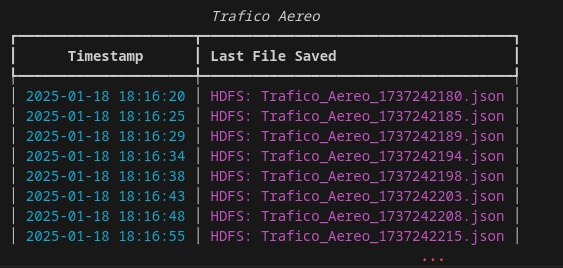
\includegraphics[width=0.8\textwidth]{terminal_output.jpg}
    \caption{Salida en consola}
\end{figure}

En paralelo a la monitorización en la terminal, el sistema también está respaldado por la web de Hadoop, que ofrece una visión detallada del estado del clúster HDFS. A través de esta interfaz web, se puede obtener información crítica sobre el estado general del sistema de archivos distribuido. La web proporciona métricas clave sobre el estado del clúster, como la cantidad de nodos activos y la distribución del almacenamiento entre los DataNodes. Esto permite a los administradores del sistema asegurarse de que todos los componentes del clúster están operando correctamente y que hay suficiente capacidad de almacenamiento disponible para manejar el volumen de datos generado.
\begin{figure}[h]
    \centering
    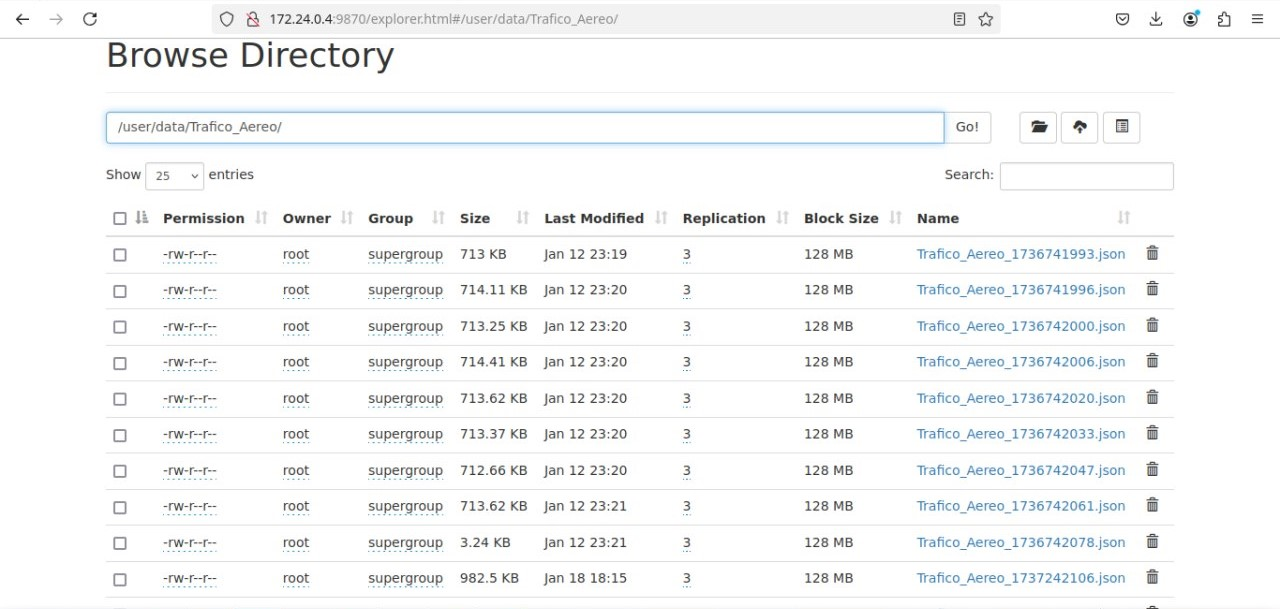
\includegraphics[width=0.9\textwidth]{HDFS_web.jpg}
    \caption{Web de hadoop}
\end{figure}

Además, la web de Hadoop ofrece detalles sobre el uso del espacio de almacenamiento en HDFS, lo que permite monitorear el crecimiento de los datos y evitar posibles cuellos de botella. Otra característica importante de la interfaz web es la capacidad de visualizar estadísticas sobre el rendimiento del sistema, como la latencia de las operaciones de lectura y escritura y el número de operaciones completadas por segundo.
Si ocurre algún problema en el clúster, la interfaz web de Hadoop muestra alertas y notificaciones, lo que permite a los administradores identificar rápidamente los problemas y tomar las acciones necesarias para resolverlos.

\section{Visualización y análisis en tiempo real}

Aunque se ha utilizado el sistema de archivos distribuidos de Hadoop para almacenar los diferentes estados de cada uno de los vuelos, hay que tener en cuenta que esta herramienta no es útil cuando se quiere acceder a los datos en tiempo real. 

A pessr de que HDFS es una excelente opción para almacenar grandes volúmenes de datos de manera distribuida y escalable, su estructura y funcionalidades están más orientadas al procesamiento por lotes y no son tan eficientes para consultas interactivas o en tiempo real. Por lo que se utilizará HDFS para poder realizar análisis teniendo en cuenta el transcurso del tiempo y para la visualización en tiempo real se utilizará otra herramienta, que será descrita a continuación. 

\subsection{Elasticsearch}
Elasticsearch es una plataforma de búsqueda y análisis de datos en tiempo real, basada en Apache Lucene \cite{Elasticsearch}. Está diseñada para ser escalable y distribuida, lo que permite gestionar grandes volúmenes de datos de manera eficiente, distribuyéndolos a través de múltiples nodos para mejorar el rendimiento y la fiabilidad.

Utiliza una estructura de datos llamada "índice invertido", donde los datos se organizan en índices, que son colecciones de documentos relacionados. Un índice es similar a una base de datos tradicional, pero optimizado para realizar búsquedas rápidas y eficientes.
En lugar de almacenar los datos en tablas, como en las bases de datos relacionales, Elasticsearch guarda la información en documentos en formato JSON. Es especialmente útil en aplicaciones donde es necesario realizar búsquedas complejas y análisis sobre conjuntos de datos en constante cambio

Para poder desplegar Elasticsearch, de conjunto con Kafka y los demás servicios, se añadió el mismo al archivo de configuración de Docker. 

\subsection{Kibana}

Kibana es una herramienta de visualización de datos que trabaja en conjunto con ElasticSearch \cite{Kibana}. Su función principal es permitir a los usuarios explorar, visualizar y compartir datos indexados en ElasticSearch de manera intuitiva y gráfica.

Toma los datos de ElasticSearch y permite representarlos en diferentes formatos visuales, como gráficos de líneas, gráficos de barras, gráficos circulares y tablas. Además, ofrece un panel interactivo donde los usuarios pueden construir y personalizar sus visualizaciones según sus necesidades específicas.

Una de las capacidades destacadas de Kibana es la creación de mapas en tiempo real mediante Elastic Maps, lo cual resulta muy útil para poder monitorear en tiempo real la posición de cada uno de los vuelos.

Además, proporciona herramientas para realizar análisis avanzados, como la creación de dashboards que combinan múltiples visualizaciones en una sola vista, lo que la hace más atractiva y brinda una mayor comprensión. 

Al igual que en el caso de Elasticsearch, se añadió el servicio de Kibana al archivo de configuración de Docker.

\subsection{Tráfico aéreo en tiempo real}
Una vez configurados Elasticsearch y Kibana en Docker, en el consumer se crea una instancia de Elasticsearch para conectarse con el servidor e iniciar la indexación. Se verifica la existencia o no, del índice y si no existe se crea, como se muestra a continuación: 

\begin{lstlisting}[style=python]
# Configuracion de Elasticsearch
ES_HOST = "http://localhost:9200"
INDEX_NAME = "air_traffic"

es = Elasticsearch([ES_HOST])
if not es.indices.exists(index=INDEX_NAME):
    mapping = {
        "mappings": {
            "properties": {
                "location": {
                    "type": "geo_point"
                }
            }
        }
    }
    es.indices.create(index=INDEX_NAME, body=mapping)
\end{lstlisting}

Luego, se procede a enviar los datos a ElasticSearch utilizando la función \textit{send\_to\_elasticsearch}, la cual valida los datos del vuelo y crea un documento con los campos relevantes, entre ellos las coordenadas geográficas. El documento es enviado a ElasticSearch para su indexación.

Una vez que los datos se encuentran en Elasticsearch, se utiliza Kibana para su visualización, herramienta a la cual se puede acceder en el navegador mediante: \url{http://localhost:5601/}. 

Como se mencionó anteriormente, con Kibana se pueden crear diferentes visualizaciones. Y en este caso se tuvo en cuenta para las mismas, la altura promedio, la velocidad promedio, las localizaciones de los aviones y  los países con la mayor cantidad de vuelos activos en el momento. Además resulta de mucha ayuda para el viajero conocer cuáles son los aeropuertos o países con mayor número de vuelos en el día, por lo también se analizó esto.

Para una mayor comprensión se creó un dashboard con todas estas visualizaciones como se muestra a continuación:

\begin{figure}[h]
    \centering
    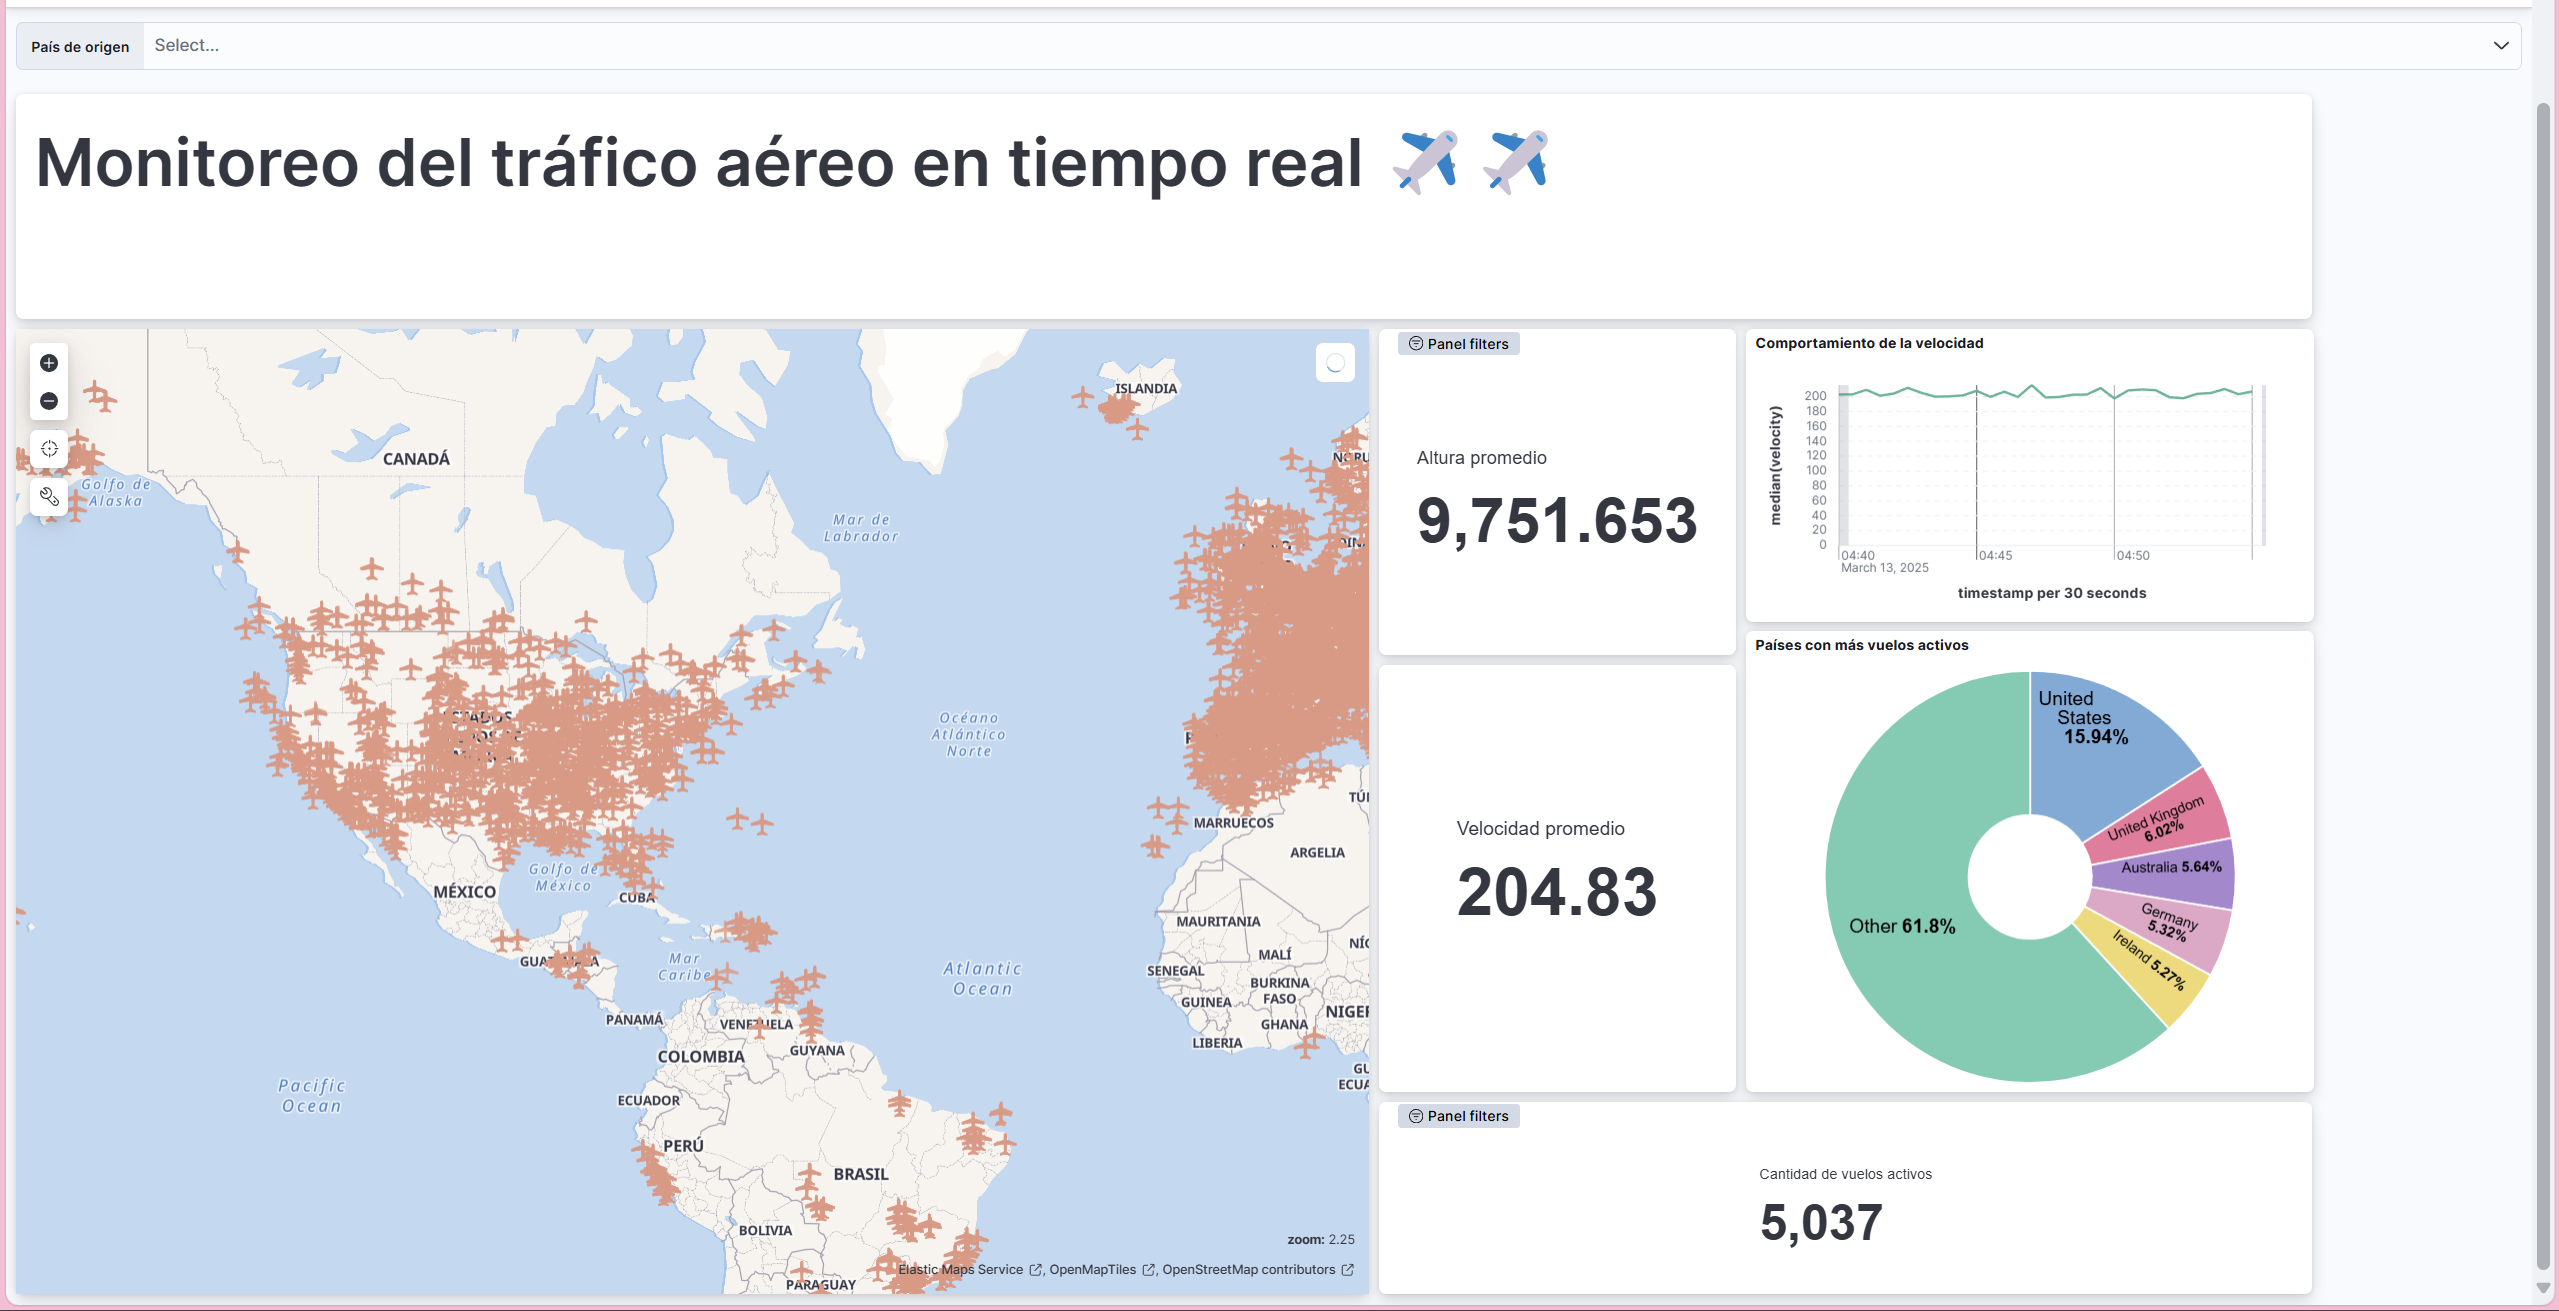
\includegraphics[width=1.0\textwidth]{traffic.png}
    \caption{Dashboard en tiempo real}
\end{figure}

\subsubsection{Predicción de retrasos}

Cuando se trata de tráfico aéreo, uno de los puntos más importantes a analizar son los aviones que, ya sea por condiciones meteorológicas u otros factores, llegan retrasados a su destino. Por esta razón, se entrenó un modelo de Machine Learning para predecir dichos retrasos. Para la predicción,se obtuvieron datos adicionales de la API de la sección de "flights", los cuales proporcionan información sobre aeropuertos de salida y de llegada, así como tiempos estimados de salida y llegada. 

Luego, con estos datos y con el objetivo de generar datos de retraso para entrenar el modelo, se calculó el tiempo que el vuelo debería demorar según la información de los aeropuertos. Posteriormente, se determinó la distancia desde la ubicación actual del avión hasta el aeropuerto de llegada, y utilizando la velocidad, se estimó el tiempo que debería demorar en llegar. Si la hora estimada de llegada es mayor en un rango superior a 15 minutos respecto a la hora programada, se considera que el avión tiene un retraso.

Con el fin de predecir retrasos en el caso de no disponer de algunos de los datos mencionados anteriormente, se utilizaron para el modelo los siguientes datos: "icao24", "longitude", "latitude", "baro\_altitude", "on\_ground", "velocity", "vertical\_rate", "geo\_altitude", "firstSeen", "lastSeen", "estDepartureAirport" y "estArrivalAirport". Estos datos se emplearon para calcular el retraso, incluyendo latitudes y longitudes, el nombre del avión, entre otros. Posteriormente, se realizaron transformaciones a los datos para poder entrenar el modelo, dividiendo los datos en conjuntos de entrenamiento y prueba, se entrenó el modelo XGBClassifier y se guardó en un archivo pickle.

El modelo XGBClassifier es una herramienta poderosa para predecir retrasos de vuelos en tiempo real ya que por una parte maneja de forma eficiente los valores faltantes y el ruido en los datos de tráfico aéreo. Además, es capaz de capturar relaciones no lineales entre múltiples factores interrelacionados, lo que resulta en una predicción más precisa de los retrasos. Este modelo también está optimizado para entrenar rápidamente en grandes volúmenes de datos. 

Una vez guardado el modelo, se utilizó FastApi para implementar un servicio web que permite hacer predicciones en tiempo real. Se cargó el modelo guardado usando la biblioteca joblib y se definió un esquema de entrada utilizando pydantic para asegurar que los datos de entrada cumplan con la estructura esperada. Se creó una ruta en la API con el método POST que recibe los datos de entrada, los transforma en un formato adecuado y pasa estos datos al modelo para obtener una predicción. Finalmente, se devuelve la predicción como parte de la respuesta JSON.
Este respuesta es incluida como otra capa del mapa usado en Kibana para la localización de los aviones, en este caso los aviones con retraso serán marcados en el mapa con otro color. 

\section{Conclusiones}

El desarrollo de este proyecto permitió implementar un sistema para la ingesta y almacenamiento de datos de tráfico aéreo en tiempo real utilizando tecnologías diseñadas para procesar grandes volúmenes de datos y transmitirlos en streaming, en lo que, la API de OpenSky Network jugó un papel fundamental para la obtención de los datos referentes al estado de las aeronaves a nivel global. 

Para asegurar una ingesta de datos eficiente y escalable, se ha integrado Apache Kafka, cuya arquitectura distribuida y tolerante a fallos maneja el flujo constante de datos sin interrupciones. Gracias a Kafka, el sistema procesa y distribuye información sobre el tráfico aéreo de manera continua, garantizando que los datos estén siempre disponibles para su análisis y almacenamiento posteriores.

La implementación de Docker y Docker Compose ha simplificado la configuración y despliegue de los servicios necesarios, permitiendo una implementación flexible y replicable en diversos entornos. Además, la integración de HDFS como sistema de almacenamiento distribuido ha proporcionado una solución para la preservación de datos históricos, asegurando su disponibilidad a largo plazo y facilitando el análisis retrospectivo.

El monitoreo del sistema se ha optimizado mediante herramientas interactivas en la terminal y la interfaz web de Hadoop, permitiendo un seguimiento del estado del clúster y del procesamiento de datos. Estas herramientas facilitan la detección temprana de problemas y garantizan un funcionamiento óptimo del sistema.

Dado que HDFS no es adecuado para consultas en tiempo real, se ha integrado Elasticsearch para indexar y buscar los datos de manera eficiente. Esta herramienta posibilita una visualización inmediata del estado de los vuelos y un análisis en tiempo real, mejorando la capacidad de monitoreo del sistema. 

No solo se visualizaron los datos geoespaciales, sino que también se implementó un modelo de Machine Learning para la predicción de retrasos en los vuelos, así como otras visualizaciones que incluyen la velocidad y altura promedio de los vuelos en cada segundo así como los países con la mayor cantidad de vuelos en tiempo real.

Todo esto, demuestra una vez más el papel que desempeña el BigData junto con todas sus herramientas para la resolución de problemas complejos. Su capacidad para procesar y analizar grandes volúmenes de datos en tiempo real no solo es clave en la aviación, sino también en muchas otras áreas, mejorando la eficiencia y la toma de decisiones.

\newpage

\begin{thebibliography}{9}

\bibitem{Schaefer2014}
Matthias Schäfer, Martin Strohmeier, Vincent Lenders, Ivan Martinovic, and Matthias Wilhelm.
\textit{Bringing Up OpenSky: A Large-scale ADS-B Sensor Network for Research}.
In Proceedings of the 13th IEEE/ACM International Symposium on Information Processing in Sensor Networks (IPSN), pages 83--94, April 2014.
\bibitem{KafkaDocumentation}
Apache Kafka.
\textit{Apache Kafka Documentation}.
Available at: \url{https://kafka.apache.org/documentation/}.
Accessed: December 2024.

\bibitem{HadoopHDFS}
Apache Hadoop.
\textit{HDFS User Guide}.
Available at: \url{https://hadoop.apache.org/docs/stable/hadoop-project-dist/hadoop-hdfs/HdfsUserGuide.html}.
Accessed: January 2025.

\bibitem{KafkaPython}
Kafka Python.
\textit{Kafka-Python Documentation}.
Available at: \url{https://kafka-python.readthedocs.io/en/master/}.
Accessed: December 2024.

\bibitem{Elasticsearch}
Elastic Documentation
\textit{Elastic Documentation}
Available at \url{https://www.elastic.co/docs}
Accessed: January 2025.

\bibitem{Kibana}
Kibana Guide
\textit{Kibana Guide}
Available at \url{https://www.elastic.co/guide/en/kibana/current/index.html}
Accessed: January 2025.
\end{thebibliography}

\end{document}